\documentclass[border=10pt]{standalone}
\usepackage{tikz}
\usepackage{amsmath}
\usepackage{amssymb}
\usetikzlibrary{positioning, arrows.meta}

% 自定义命令
\newcommand{\ket}[1]{|#1\rangle}

\begin{document}
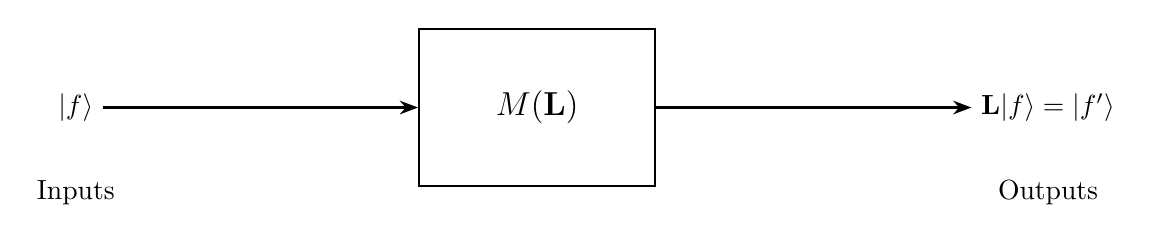
\begin{tikzpicture}[
    node distance = 3cm,
    auto,
    % 样式定义
    sysblock/.style = {
        rectangle,
        draw = black,
        fill = white,
        minimum width = 3cm,
        minimum height = 2cm,
        line width = 0.8pt,
        font = \large
    },
    label/.style = {
        font = \normalsize
    }
]

% 节点定义
\node[sysblock] (system) {$M(\mathbf{L})$};

\node[label, left = 4cm of system] (input_signal) {$\ket{f}$};
\node[label, below = 0.5cm of input_signal] (input_label) {Inputs};

\node[label, right = 4cm of system] (output_signal) {$\mathbf{L}\ket{f} = \ket{f'}$};
\node[label, below = 0.5cm of output_signal] (output_label) {Outputs};

% 连接线
\draw[->, >=Stealth, line width = 0.8pt] 
    (input_signal) -- (system.west);
\draw[->, >=Stealth, line width = 0.8pt] 
    (system.east) -- (output_signal);

\end{tikzpicture}
\end{document}